\documentclass{article}
\usepackage{mathtools}% loads `amsmath'
\usepackage{newtxtext,tikz,pgfplots}
\usepackage[scaled=0.861,lining]{FiraMono}
\pgfplotsset{width=7cm,compat=1.8}
\usepgfplotslibrary{polar}


\def\bracesshape{curlybraces}% change here to obtain different braces
% curlybraces
% morphedbraces
% straightbraces
\usepackage[lite,\bracesshape]{mtpro2}

% Patches begin
\makeatletter
\newsavebox{\mtp@casesbox}
% Activate `mathtools' syntax
\MHInternalSyntaxOn
% Curly braces are used only if `curlybraces' is set
% From `mtpro2.sty': \DeclareOption{curlybraces}{\let\mtp@br=c}
\MH_if_meaning:NN \mtp@br c
  \expandafter\@firstofone
\MH_else:
  \expandafter\@gobble
\MH_fi:{
  \def\MTP_MT_start_cases:nnn #1#2#3{ % #1=sep,#2=lpreamble,#3=rpreamble
   \RIfM@\else
     \nonmatherr@{\begin{\@currenvir}}
   \fi
   \MH_group_align_safe_begin:
   \setbox\mtp@casesbox=\hbox\bgroup$% <- put contents in `\mtp@casesbox'
   \vcenter \bgroup
       \Let@ \chardef\dspbrk@context\@ne \restore@math@cr
       \let  \math@cr@@\AMS@math@cr@@
       \spread@equation
       \ialign\bgroup
         \strut@#2 &#1\strut@
         #3
         \crcr
  }
  \def\MTP_MH_end_cases:{\crcr\egroup
   \restorecolumn@
   \egroup
   $\egroup% <- close the `\hbox'
   \MH_group_align_safe_end:
  }
  \newcommand*\mtp@newcases[6]{% #1=name, #2=sep, #3=lpreamble, #4=rpreamble, #5=left, #6=right
   \newenvironment{#1}
     {\MTP_MT_start_cases:nnn {#2}{#3}{#4}}
     {\MTP_MH_end_cases:\LEFTRIGHT#5#6{\copy\mtp@casesbox}}
  }
  \newcommand*\mtp@renewcases[6]{
   \renewenvironment{#1}
     {\MTP_MT_start_cases:nnn {#2}{#3}{#4}}
     {\MTP_MH_end_cases:\LEFTRIGHT#5#6{\copy\mtp@casesbox}}
  }
  \mtp@renewcases{dcases}{\quad}{%
    $\m@th\displaystyle{##}$\hfil}{$\m@th\displaystyle{##}$\hfil}{\lbrace}{.}
  \mtp@renewcases{dcases*}{\quad}{%
    $\m@th\displaystyle{##}$\hfil}{{##}\hfil}{\lbrace}{.}
  \mtp@newcases{cdcases}{\quad}{%
    $\m@th\hfil\displaystyle{##}$\hfil}{$\m@th\displaystyle{##}$\hfil}{\lbrace}{.}
  \mtp@newcases{cdcases*}{\quad}{%
    $\m@th\hfil\displaystyle{##}$\hfil}{{##}\hfil}{\lbrace}{.}
  \mtp@renewcases{rcases}{\quad}{%
    $\m@th{##}$\hfil}{$\m@th{##}$\hfil}{.}{\rbrace}
  \mtp@renewcases{rcases*}{\quad}{%
    $\m@th{##}$\hfil}{{##}\hfil}{.}{\rbrace}
  \mtp@renewcases{drcases}{\quad}{%
    $\m@th\displaystyle{##}$\hfil}{$\m@th\displaystyle{##}$\hfil}{.}{\rbrace}
  \mtp@renewcases{drcases*}{\quad}{%
    $\m@th\displaystyle{##}$\hfil}{{##}\hfil}{.}{\rbrace}
  \mtp@renewcases{cases*}{\quad}{%
    $\m@th{##}$\hfil}{{##}\hfil}{\lbrace}{.}
}
% Deactivate `mathtools' syntax
\MHInternalSyntaxOff
\makeatother
% Patches end

\newcommand*\showopendelimitersizes[1]{%
  #1\bigl#1\Bigl#1\biggl#1\Biggl#1}

\begin{document}

\section*{\texttt{dcases*} in \texttt{align} work?}
\verb|dcases*| and friends from \verb|mathtools| work,
iff \verb|curlybraces| is set.
\subsection*{Package \texttt{mtpro2} options: \texttt{lite,\bracesshape}}
\begin{align*}
%\showopendelimitersizes{\lbrace}
\begin{cdcases*}
\int_a^b f(x) \, \mathrm{d}x    & Nothing to see here \\
\sum_{n=1}^\infty \frac{1}{n^2} & Otherwise
\end{cdcases*}
\end{align*}
With \verb|morphedbraces| or \verb|straightbraces|,
errors appear.
\newcommand{\gwnia}[5][]{
\fill[#1](#4:#2-#3) --(#4:#2) arc (#4:#5:#2)--(#5:#2-#3) arc (#5:#4:#2-#3);
}

\begin{tikzpicture}
\draw[-latex] (-2,0) -- (2,0) coordinate (xaxis);
\draw[-latex] (0,-1.5) -- (0,2) coordinate (yaxis);
\gwnia[cyan,opacity=0.7]{1}{0.4}{0}{200}
\gwnia[magenta,opacity=0.7]{1.4}{0.4}{40}{200}
\gwnia[yellow!55!green!70,opacity=0.8]{1.8}{0.4}{20}{150}
\gwnia[orange!70,opacity=0.8]{.6}{0.4}{40}{250}
\end{tikzpicture}
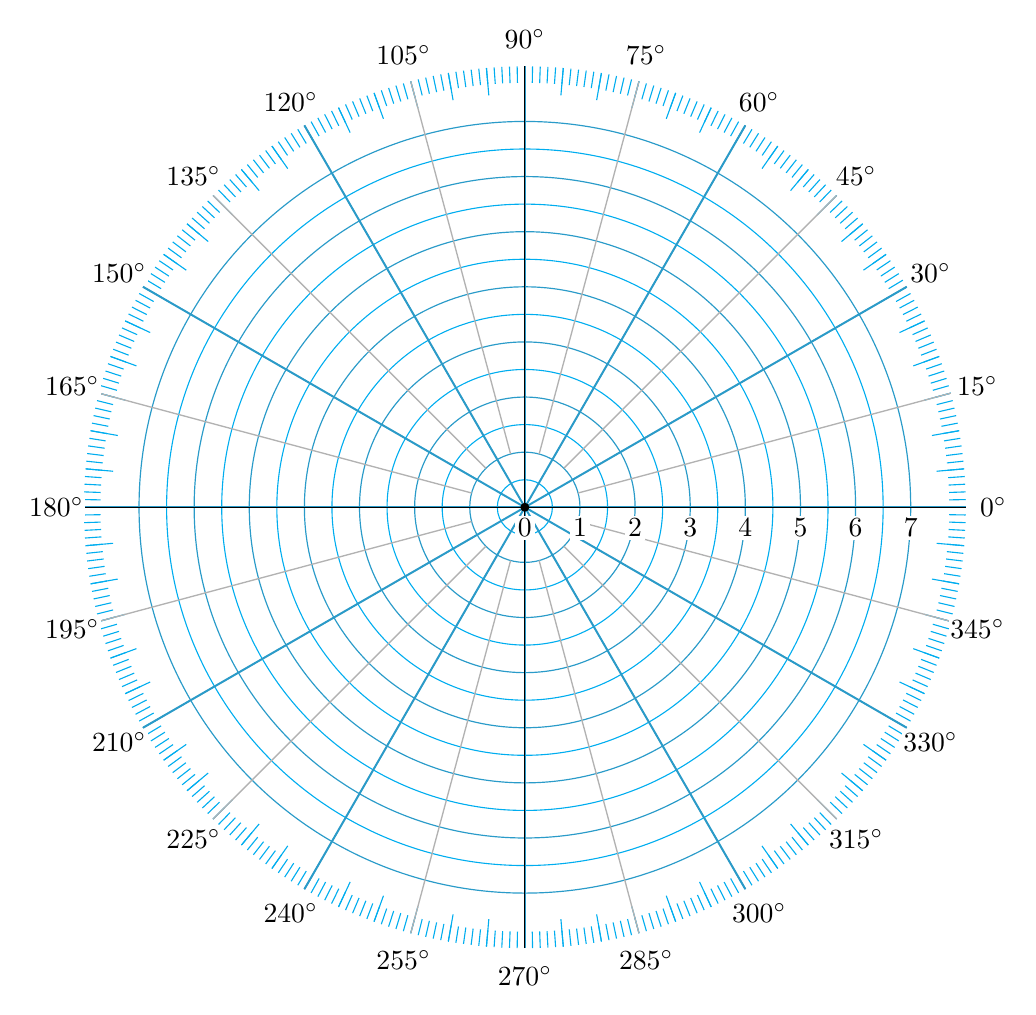
\begin{tikzpicture}[scale=0.7]
%Circles 
\foreach \r in {1, 2,...,7}
\draw[cyan!80!black, line width=.15mm] (0,0) circle (\r);    
\foreach \r in {0.5, 1.5,...,7}
\draw[cyan, thin] (0,0) circle (\r);
%1° Rays
\foreach \a in {0, 1,...,359}
\draw[cyan] (\a:7.7) -- (\a:8);
%5° Rays
\foreach \a in {0, 5,...,359}
\draw[cyan] (\a:7.5) -- (\a:8);      
%15° Rays
\foreach \a in {0, 15,...,359}
\draw[line width=.17mm,black!30] (\a:1) -- (\a:8); 
%30° Rays
\foreach \a in {0, 30,...,359}
\draw[line width=.25mm,cyan!80!black] (0, 0) -- (\a:8);
%Main rays
\draw (-8,0) -- (8,0);
\draw (0,-8) -- (0,8);
%Angle labels  
\foreach \a in {0, 15,...,359}
\draw (\a: 8.5) node[fill=white,inner sep=.2mm] {$\a^\circ$};
%Central point
\draw[fill=black] (0,0) circle(0.7mm);
%Radius labels (background filled white)
\foreach \r in {0,1,...,7}
\draw (\r,0) node[inner sep=1pt,below=3pt,rectangle,fill=white] {$\r$};
\end{tikzpicture}
\end{document}